\documentclass[letterpaper, 10 pt, conference]{latex_template/ieeeconf}

\overrideIEEEmargins

\usepackage[utf8]{inputenc}
\usepackage[T1]{fontenc}
\usepackage{graphics}
\usepackage{graphicx}
\usepackage{amsmath}
\usepackage{amssymb}

% ieeeconf usa \fnum@table (no \tablename) para el label de tablas
% y ya define \fnum@figure como "Fig.~\thefigure" con numeración arábiga
\AtBeginDocument{%
  \def\fnum@table{Tabla~\thetable}%
  \renewcommand{\thetable}{\arabic{table}}%
}

\title{\LARGE \bf
Clasificación de Artículos de Noticias de la BBC usando Transformers
}

\author{Yezid Garcia$^{1}$, Juan Martin Santos$^{1}$ y Jaime Rodriguez$^{1}$ \\
{\small $^{1}$Universidad de los Andes, Bogotá, Colombia} \\
{\small Códigos: 200810710, 202013610, 200717791}
}

\begin{document}

\maketitle
\thispagestyle{empty}
\pagestyle{empty}

%%%%%%%%%%%%%%%%%%%%%%%%%%%%%%%%%%%%%%%%%%%%%%%%%%%%%%%%%%%%%%%%%%%%%%%%%%%%%%%%
\section{Introducción}

La arquitectura transformer, propuesta por Vaswani et al. \cite{c1}, reemplaza las redes recurrentes por mecanismos de atención que relacionan cualquier par de posiciones de una secuencia en tiempo constante. Este diseño elimina la dependencia secuencial de las LSTM y permite paralelizar el entrenamiento sobre secuencias largas. Sobre esta base, Devlin et al. \cite{c2} desarrollaron BERT, un modelo preentrenado mediante predicción de tokens enmascarados en grandes corpus no etiquetados, cuyo ajuste fino sobre tareas específicas establece resultados de referencia en clasificación de texto, extracción de información y preguntas y respuestas. En paralelo, Radford et al. \cite{c3} demostraron con GPT que el preentrenamiento autorregresivo seguido de fine-tuning también generaliza bien a múltiples tareas de comprensión del lenguaje.

La clasificación automática de noticias presenta el reto de asignar categorías temáticas a textos de longitud variable con solapamiento semántico entre dominios. El corpus BBC News \cite{c4}, con 2225 artículos en cinco categorías, es un banco de prueba estándar para este problema: un artículo de política económica comparte términos con noticias de negocios; una crónica deportiva con cifras puede confundirse con contenido financiero. Las soluciones basadas en bolsa de palabras pierden el orden y el contexto necesarios para resolver estas ambigüedades.

En este trabajo se implementa un clasificador sobre el corpus BBC News usando DistilBERT \cite{c5}, versión destilada de BERT que conserva el 97\% de su rendimiento con la mitad de parámetros. El modelo se ajusta mediante fine-tuning durante cinco épocas. El documento describe los datos, la arquitectura, el procedimiento de entrenamiento, los resultados cuantitativos con curvas de entrenamiento, los resultados cualitativos y una discusión sobre limitaciones y trabajo futuro.

%%%%%%%%%%%%%%%%%%%%%%%%%%%%%%%%%%%%%%%%%%%%%%%%%%%%%%%%%%%%%%%%%%%%%%%%%%%%%%%%
\section{Metodología}

\subsection{Datos}

Se utiliza el conjunto BBC News \cite{c4}, compuesto por 2225 artículos periodísticos en cinco categorías: \textit{business} (510), \textit{entertainment} (386), \textit{politics} (417), \textit{sport} (511) y \textit{tech} (401). Cada entrada contiene el titular y el cuerpo del texto como cadena plana. El conjunto no presenta valores nulos ni duplicados.

Los datos se dividen de forma estratificada en tres subconjuntos: entrenamiento (70\%, 1557 artículos), validación (15\%, 334 artículos) y prueba (15\%, 334 artículos). La partición estratificada preserva la proporción de categorías en cada subconjunto.

\subsection{Preprocesamiento}

El texto se tokeniza con el vocabulario WordPiece de DistilBERT, que descompone las palabras en subpalabras frecuentes del corpus de preentrenamiento. A cada secuencia se agregan los tokens especiales \texttt{[CLS]} al inicio y \texttt{[SEP]} al final, siguiendo el esquema de BERT \cite{c2}. Las secuencias se truncan o rellenan hasta 256 tokens. Una máscara de atención binaria indica cuáles posiciones corresponden a contenido real. Las etiquetas de categoría se codifican como enteros del 0 al 4. La tokenización del conjunto completo se ejecuta una sola vez antes del entrenamiento para evitar cómputo redundante en cada época.

\subsection{Arquitectura}

El modelo se organiza en dos bloques, siguiendo el esquema de clasificación de secuencias de BERT \cite{c2}. El primer bloque es DistilBERT \cite{c5}, que procesa la secuencia mediante seis capas de atención multi-cabeza y produce una representación contextual para cada posición. La representación del token \texttt{[CLS]} —que agrega el contexto global de la secuencia— se extrae como vector de 768 dimensiones. El segundo bloque es una capa de clasificación lineal que proyecta este vector sobre cinco clases y aplica softmax. El modelo tiene aproximadamente 67 millones de parámetros.

\subsection{Entrenamiento y métricas}

El modelo se entrena durante cinco épocas con el optimizador AdamW con tasa de aprendizaje inicial $2 \times 10^{-5}$. Se aplica un scheduler lineal con calentamiento en el 10\% de los pasos totales, lo que reduce la magnitud de las actualizaciones iniciales y estabiliza el ajuste fino de los pesos preentrenados. El gradiente se recorta a norma máxima 1.0 antes de cada actualización. El tamaño de lote es 16. Se guarda el checkpoint con menor pérdida de validación, que se usa para la evaluación final.

Las métricas de evaluación son precisión, recall y F1-score por categoría, y exactitud global sobre el conjunto de prueba.

%%%%%%%%%%%%%%%%%%%%%%%%%%%%%%%%%%%%%%%%%%%%%%%%%%%%%%%%%%%%%%%%%%%%%%%%%%%%%%%%
\section{Resultados}

\subsection{Resultados cuantitativos}

La Tabla 1 presenta los resultados sobre el conjunto de prueba (334 artículos). El modelo alcanza una exactitud global de \textbf{97.90\%} (327/334) y un F1-score macro de 0.979.

\begin{table}[h]
\centering
\caption{Precisión, recall y F1-score por categoría en el conjunto de prueba.}
\resizebox{8.5cm}{!}{
\begin{tabular}{|l|c|c|c|c|}
\hline
\textbf{Categoría} & \textbf{Precisión} & \textbf{Recall} & \textbf{F1} & \textbf{Soporte} \\ \hline
business           & 0.9610 & 0.9610 & 0.9610 & 77 \\ \hline
entertainment      & 0.9828 & 0.9828 & 0.9828 & 58 \\ \hline
politics           & 0.9672 & 0.9516 & 0.9593 & 62 \\ \hline
sport              & 1.0000 & 1.0000 & 1.0000 & 77 \\ \hline
tech               & 0.9836 & 1.0000 & 0.9917 & 60 \\ \hline
\textbf{macro avg} & \textbf{0.9789} & \textbf{0.9791} & \textbf{0.9790} & \textbf{334} \\ \hline
\end{tabular}}
\end{table}

Como se observa en la Tabla 1, \textit{sport} obtuvo clasificación perfecta (F1 = 1.0) y \textit{tech} obtuvo recall perfecto (1.0) con precisión de 0.9836. La categoría \textit{politics} presentó el F1 más bajo (0.9593) con recall de 0.9516, indicando que algunos artículos de política se asignaron a otras categorías.

La Fig. 1 muestra las curvas de pérdida y exactitud durante el entrenamiento. La pérdida de validación desciende de forma consistente durante las primeras épocas y se estabiliza, lo que indica convergencia sin sobreajuste dentro del rango de cinco épocas. La incorporación del scheduler con calentamiento y el recorte de gradiente —ausentes en una versión previa del pipeline— redujo la varianza de la pérdida entre épocas, produciendo curvas más regulares.

\begin{figure}[h]
    \centering
    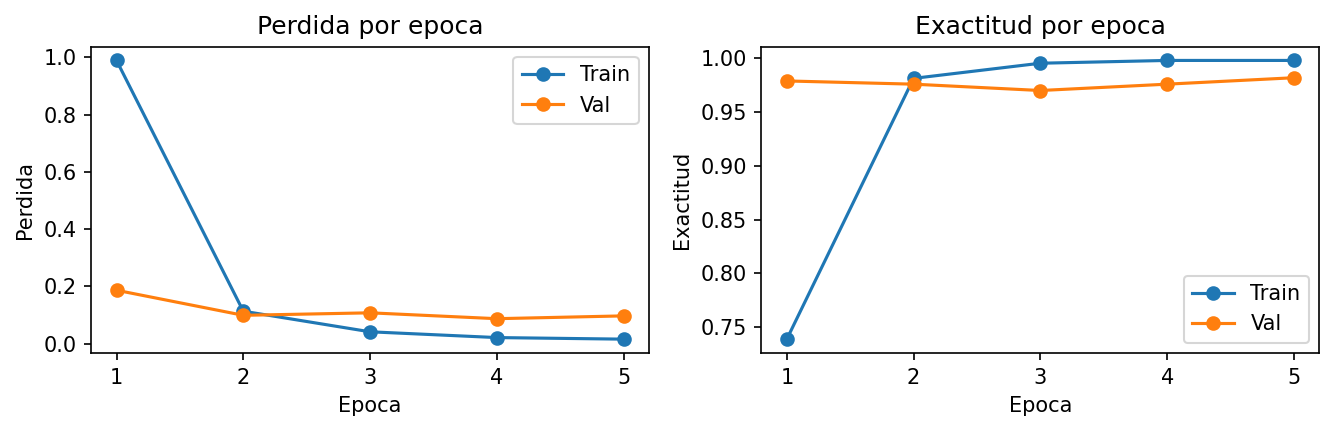
\includegraphics[width=0.98\linewidth]{training_curves.png}
    \caption{Curvas de pérdida (izquierda) y exactitud (derecha) por época sobre los conjuntos de entrenamiento y validación. Generadas desde el notebook de entrenamiento.}
\end{figure}

\subsection{Resultados cualitativos}

El modelo diferencia con mayor facilidad las categorías con vocabulario específico. \textit{Sport} concentra términos de dominio deportivo —nombres de competencias, marcadores, equipos— que no aparecen en otras categorías. \textit{Tech} incluye términos de tecnología cuya precisión de 0.9836 menor que 1.0 sugiere que algunos artículos de otras categorías con contenido tecnológico se clasificaron en esta clase.

\textit{Politics} es la categoría de mayor dificultad. Artículos sobre política económica o regulación tecnológica comparten vocabulario con \textit{business} y \textit{tech}. El mecanismo de atención de DistilBERT captura relaciones de largo alcance entre palabras del texto, lo que permite resolver la mayoría de estas ambigüedades a partir de la representación del token \texttt{[CLS]}. Los siete artículos clasificados incorrectamente corresponden en su mayoría a este tipo de solapamiento temático.

%%%%%%%%%%%%%%%%%%%%%%%%%%%%%%%%%%%%%%%%%%%%%%%%%%%%%%%%%%%%%%%%%%%%%%%%%%%%%%%%
\section{Discusión}

El resultado de 97.90\% de exactitud con cinco épocas de fine-tuning sobre 2225 documentos ilustra la efectividad del aprendizaje por transferencia introducido por BERT \cite{c2} y GPT \cite{c3}. DistilBERT \cite{c5}, preentrenado sobre grandes corpus mediante predicción de tokens enmascarados, captura estructura sintáctica y semántica del lenguaje sin requerir etiquetas de tarea. El ajuste fino sobre el corpus BBC orienta esta representación general hacia la clasificación temática en pocas épocas, lo que confirma el principio demostrado también por T5 \cite{c6} y GPT-3 \cite{c7}: el costo de adaptación a un dominio específico se reduce sustancialmente al partir de pesos preentrenados en texto general.

La arquitectura transformer \cite{c1} presenta ventajas frente a redes recurrentes para texto periodístico. Su atención global permite relacionar el titular con información de párrafos posteriores del artículo e integrar señales distribuidas a lo largo del documento. En el caso de \textit{politics}, aunque los artículos comparten vocabulario con otras categorías, la representación contextual del token \texttt{[CLS]} contiene señales suficientes para la clasificación correcta en el 95.16\% de los casos.

Entre las limitaciones del trabajo se encuentran el tamaño del conjunto (2225 artículos), la ausencia de una línea base cuantitativa como clasificación sobre representaciones TF-IDF o DistilBERT con backbone congelado sin fine-tuning, y la falta de un estudio de ablación que aísle el efecto individual del scheduler y el recorte de gradiente. Como trabajo futuro se propone comparar el fine-tuning completo frente a la extracción de características con backbone congelado, evaluar el modelo en corpus de noticias de otras fuentes para medir generalización entre dominios, y realizar un análisis de errores por categoría que identifique los patrones léxicos asociados a las confusiones en \textit{politics}.

\begin{thebibliography}{99}

\bibitem{c1} A. Vaswani, N. Shazeer, N. Parmar, J. Uszkoreit, L. Jones, A. N. Gomez, L. Kaiser e I. Polosukhin, ``Attention Is All You Need,'' en \textit{Advances in Neural Information Processing Systems (NeurIPS)}, vol. 30, 2017.

\bibitem{c2} J. Devlin, M.-W. Chang, K. Lee y K. Toutanova, ``BERT: Pre-training of Deep Bidirectional Transformers for Language Understanding,'' en \textit{Proc. NAACL-HLT}, págs. 4171--4186, 2019.

\bibitem{c3} A. Radford, K. Narasimhan, T. Salimans e I. Sutskever, ``Improving Language Understanding by Generative Pre-Training,'' \textit{Technical Report}, OpenAI, 2018.

\bibitem{c4} D. Greene y P. Cunningham, ``Practical Solutions to the Problem of Diagonal Dominance in Kernel Document Clustering,'' en \textit{Proc. 23rd Int. Conf. Machine Learning (ICML)}, págs. 377--384, 2006.

\bibitem{c5} V. Sanh, L. Debut, J. Chaumond y T. Wolf, ``DistilBERT, a distilled version of BERT: smaller, faster, cheaper and lighter,'' \textit{arXiv preprint arXiv:1910.01108}, 2019.

\bibitem{c6} C. Raffel, N. Shazeer, A. Roberts, K. Lee, S. Narang, M. Matena, Y. Zhou, W. Li y P. J. Liu, ``Exploring the Limits of Transfer Learning with a Unified Text-to-Text Transformer,'' \textit{Journal of Machine Learning Research}, vol. 21, núm. 140, págs. 1--67, 2020.

\bibitem{c7} T. B. Brown et al., ``Language Models are Few-Shot Learners,'' en \textit{Advances in Neural Information Processing Systems (NeurIPS)}, vol. 33, 2020.

\end{thebibliography}

\end{document}
